\documentclass[11pt,spanish,a4paper]{article}
% Versión 1.er cuat 2021 Víctor Bettachini < bettachini@df.uba.ar >

% Versión 1.er cuat 2021 Víctor Bettachini < bettachini@df.uba.ar >

\usepackage[T1]{fontenc}
\usepackage[utf8]{inputenc}

\usepackage[spanish, es-tabla]{babel}
\def\spanishoptions{argentina} % Was macht dass?
% \usepackage{babelbib}
% \selectbiblanguage{spanish}
% \addto\shorthandsspanish{\spanishdeactivate{~<>}}

\usepackage{graphicx}
\graphicspath{{./figuras/}}
% \usepackage{float}

\usepackage[arrowdel]{physics}
\newcommand{\pvec}[1]{\vec{#1}\mkern2mu\vphantom{#1}}
% \usepackage{units}
\usepackage[separate-uncertainty=true, multi-part-units=single, locale=FR]{siunitx}
\usepackage{isotope} % $\isotope[A][Z]{X}\to\isotope[A-4][Z-2]{Y}+\isotope[4][2]{\alpha}

\usepackage{tasks}
\usepackage[inline]{enumitem}
% \usepackage{enumerate}

\usepackage{hyperref}

% \usepackage{amsmath}
% \usepackage{amstext}
\usepackage{amssymb}

\usepackage{tikz}
\usepackage{tikz-dimline}
\usetikzlibrary{math}
\usetikzlibrary{arrows.meta}
% \usetikzlibrary{snakes}
% \usetikzlibrary{calc}
\usetikzlibrary{decorations.pathmorphing}
\usetikzlibrary{patterns}

\usepackage[hmargin=1cm,vmargin=1.6cm,nohead]{geometry}
% \voffset-3.5cm
% \hoffset-3cm
% \setlength{\textwidth}{17.5cm}
% \setlength{\textheight}{27cm}

\usepackage{lastpage}
\usepackage{fancyhdr}
\pagestyle{fancyplain}
\fancyhead{}
\fancyfoot{{\tiny \textcopyright DF, FCEyN, UBA}}
\fancyfoot[C]{ {\tiny Actualizado al \today} }
\fancyfoot[RO, LE]{Pág. \thepage/\pageref{LastPage}}
\renewcommand{\headrulewidth}{0pt}
\renewcommand{\footrulewidth}{0pt}


\begin{document}
\begin{center}
\textbf{Física 2} (Físicos) \hfill \textcopyright {\tt DF, FCEyN, UBA}\\
	\textsc{\LARGE Reflexión y transmisión de ondas}
\end{center}

Los ejercicios con (*) son opcionales.

\begin{enumerate}

\item Nos interesa estudiar la unión de dos cuerdas de distinta densidad lineal $\rho_1$ y $\rho_2$, por lo que las consideraremos semi--infinitas. 
Mientras se las somete a una tensión $T$ constante incide desde la primera una onda $\Psi_i(x,t) = A_i \cos{ \left( k_{1} x- \omega t \right) }$.
Se conocen $\rho_{1}$, $\rho_{2}$, $T$, $\omega$ y $A_{i}$.
\begin{enumerate}
	\item Calcule $k_{1}$ y $k_{2}$, es decir, los números de onda de cada lado de la unión.
	\item Plantee la solución más general para $\Psi(x,t)$ de cada lado de la unión.
	\item ¿Qué condiciones deben verificarse en el punto de unión de las cuerdas?
	\item Usando b) y c), calcule la perturbación $\Psi(x,t)$ en cada una de las cuerdas.
\end{enumerate}


\item
\begin{minipage}[t][3.3cm]{0.6\textwidth}
Como nos interesa estudiar la unión de dos caños cuadrados de área transversal $A_1$ y $A_2$ los consideramos semi--infinitos.
Desde el izquierdo incide una onda acústica $\delta p_i (x,t) = a_i \cos{ \left( k_i x - \omega t \right) }$.
Suponga despreciables los efectos de la viscosidad y dé por conocidos $A_{1}$, $A_{2}$, presión media $P_{0}$, densidad media $\rho_{0}$, $v_{s}$, $\omega$, $a_i$.
Halle amplitudes de presión y desplazamiento de moléculas a causa de las ondas reflejadas y transmitidas.
\end{minipage}
\begin{minipage}[c][0cm][t]{0.34\textwidth}
	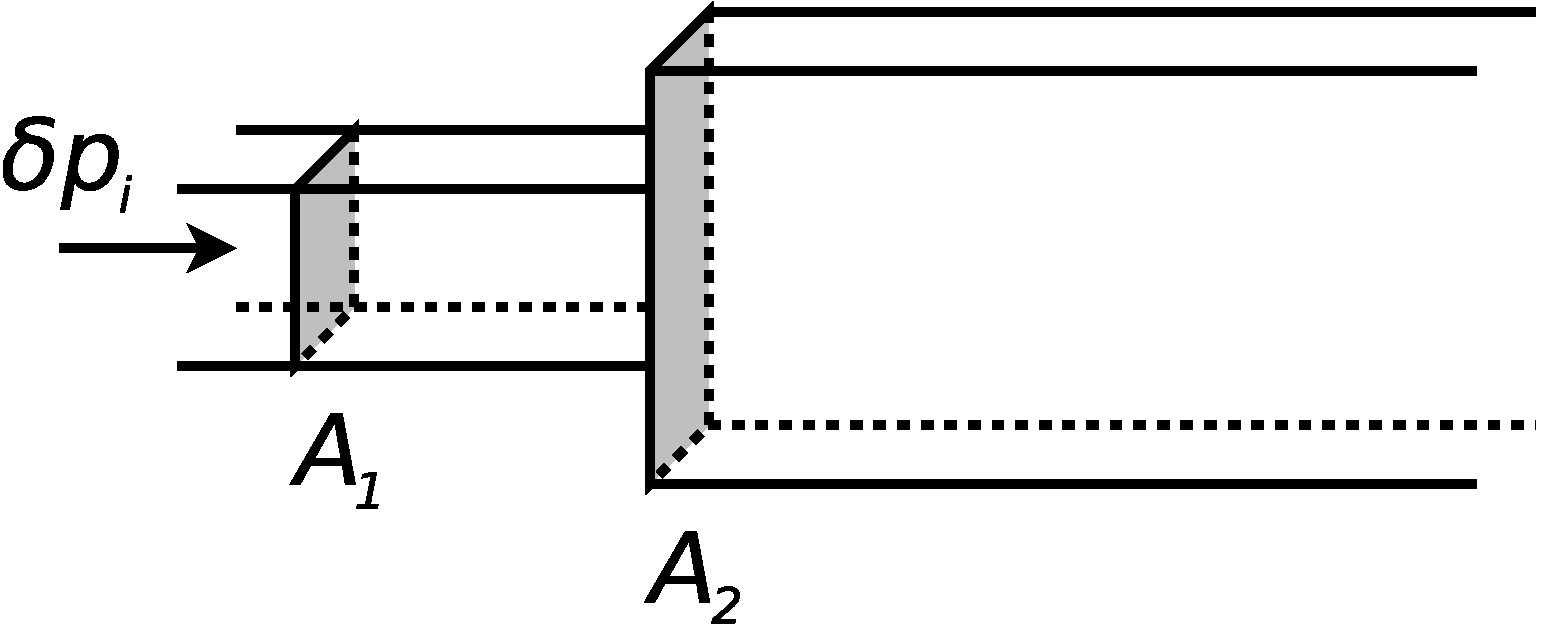
\includegraphics[width=\textwidth]{ej2-10}
\end{minipage}


\item 
\begin{minipage}[t][1.6cm]{0.6\textwidth}
A este armado con idénticas áreas del problema anterior incide la misma onda.
Halle $\delta p(x,t)$ y $\Psi(x,t)$ en cada tramo.
\end{minipage}
\begin{minipage}[c][1cm][t]{0.34\textwidth}
	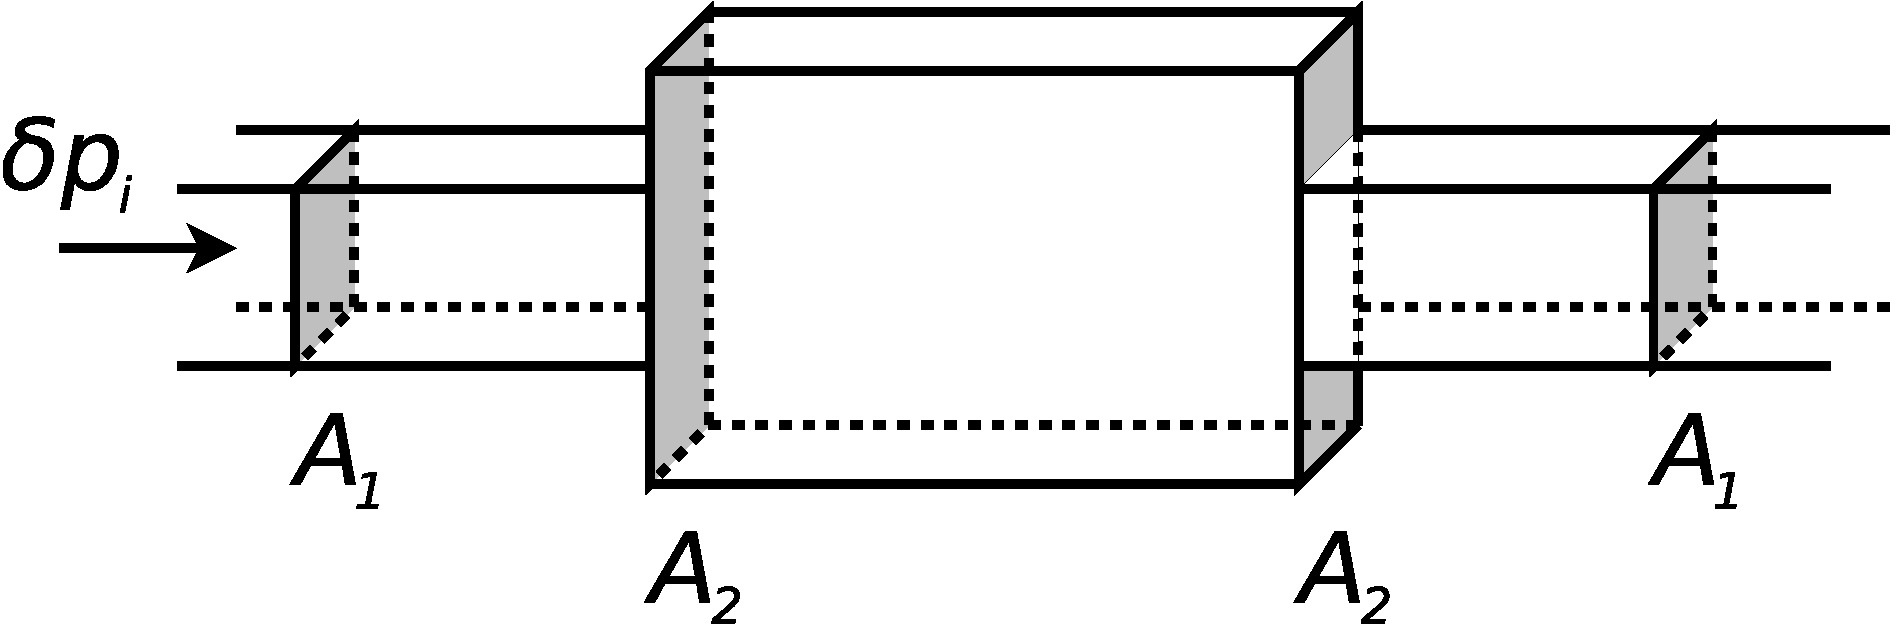
\includegraphics[width=\textwidth]{ej2-11}
\end{minipage}


\item
Desde el aire incide en dirección perpendicular a una superficie calma de agua una onda de sonido plana $\delta p_i (y,t) = A_i \cos{\left( k_i y - \omega t \right)}$.
Hallar la onda reflejada $\delta p_{r}(y,t)$ y transmitida $\delta p_{t}(y,t)$.
\begin{figure}[ht]
\centering{}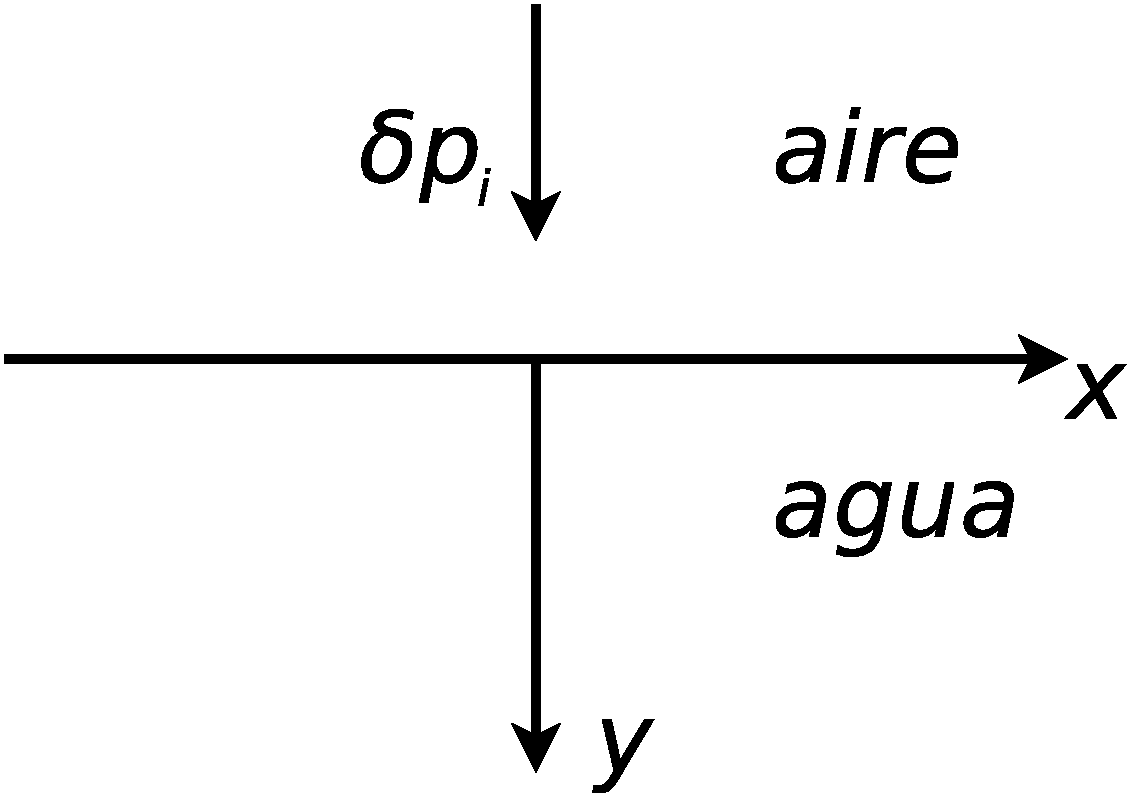
\includegraphics[clip,scale=0.25]{ej2-12}
\end{figure}




\end{enumerate}

\end{document}
